\documentclass{boi2014-et}

\renewcommand{\DayNum}{2}
\renewcommand{\TaskCode}{postmen}
\renewcommand{\TaskName}{Eakad postiljonid}

\begin{document}

    \begin{wrapfigure}[8]{r}{4cm}
        \vspace{-18pt}
        \includegraphics[width=4cm]{\TaskCode.jpeg}
    \end{wrapfigure}

    On aasta 2036 ja Euroopa on täis eakaid kodanikke.
    Et neid tervena hoida, pakkus Euroopa enamusgruppide ministeerium
    (eakad \emph{on} enamus!) välja idee rakendada neid postiljonidena,
    et toimetada kohale need vähesed paberkirjad, mida veel saadetakse
    (enamasti eakatele).
    Nüüd hakataksegi seda ideed üle Euroopa ellu viima.

    Selleks on ministeerium kujundanud ``eakate postiljonide süsteemi''
    järgmiselt:
    Euroopa on jagatud postikandepiirkondadeks. Iga piirkonna tänavavõrk
    koosneb ristmikest ja neid ühendavatest kahesuunalistest tänavatest.
    Igas piirkonnas on praktiliselt piiramatu arv eakaid, keda võiks
    postiljonidena tööle võtta. Igal hommikul saab iga postiljon koti
    kirjadega, mis tuleb kanda laiali postiringil, mis katab osa selle
    kandepiirkonna tänavavõrgust. Iga postiring peab olema eakasõbralik,
    s.t. rahuldama järgmisi tingimusi:
    \begin{itemize}
        \item Ring lõpeb samal ristmikul, millelt ta algab.
        \item Üks ring ei läbi ühtegi ristmikku korduvalt.
            (Eakaid ei tohi segadusse ajada.)
        \item Mitte mingid kaks ringi ei läbi sama tänavat;
            teisisõnu, piirkonna igal tänaval on täpselt üks postiljon.
            (Eakad ei pea üksteisega võistlema.)
    \end{itemize}

    Kõik postiringid kokku peavad katma kogu tänavavõrgu: iga tänav peab
    kuuluma täpselt ühe postiringi koosseisu.

    \Task

    Ministeeriumil on nüüd vaja programmi, mis koostab antud tänavavõrgule
    seda katva eaka\-sõbralike postiringide süsteemi.

    \Input

    Sisend kirjeldab ühe postikandepiirkonna tänavavõrku.

    Sisendi esimesel real on täisarvud $N$ ja $M$, kus $N$ on ristmike ja
    $M$ tänavate arv. Ristmikud on nummerdatud $1 \ldots N$.

    Järgmisel $M$ real on igaühel täisarvud $u$ ja $v$ ($1 \le u, v \le N$,
    $u \ne v$), mis näitavad, et ristmike $u$ ja $v$ vahel on tänav.

    Tänavavõrk rahuldab järgmisi tingimusi:
    \begin{enumerate}
        \item Mitte mingit kaht ristmikku ei ühenda rohkem kui üks tänav.
        \item Igalt ristmikult pääseb igale teisele ristmikule,
            läbides selleks ühe või mitu tänavat.
        \item Leidub vähemalt üks eakasõbralik postiringide süsteem.
    \end{enumerate}

    \Output

    Väljundi iga rida peab kirjeldama üht postiringi, loetledes ristmikud,
    mida see ring läbib. Ristmikud tuleb loetleda nende läbimise järjekorras.
    Ringi algusristmik (mis on ühtlasi ka ringi lõpp) väljastada esimesena
    (ja ainult üks kord).

    Kui võimalikke lahendusi on mitu, väljastada ükskõik milline neist.

    \Example

    \example
    {
        10 15 \newline
        1 3 \newline
        5 1\newline
        2 3 \newline
        9 2\newline
        3 4 \newline
        6 3\newline
        4 5 \newline
        7 4\newline
        4 8 \newline
        5 7 \newline
        8 5\newline
        6 7 \newline
        7 8 \newline
        8 10 \newline
        10 9
    }
    {
        2 3 4 5 8 10 9 \newline
        7 8 4 \newline
        1 5 7 6 3
    }
    {
        Järgnev joonis illustreerib tänavavõrku ja kolme eakasõbralikku
        postiringi, mis selle katavad.

        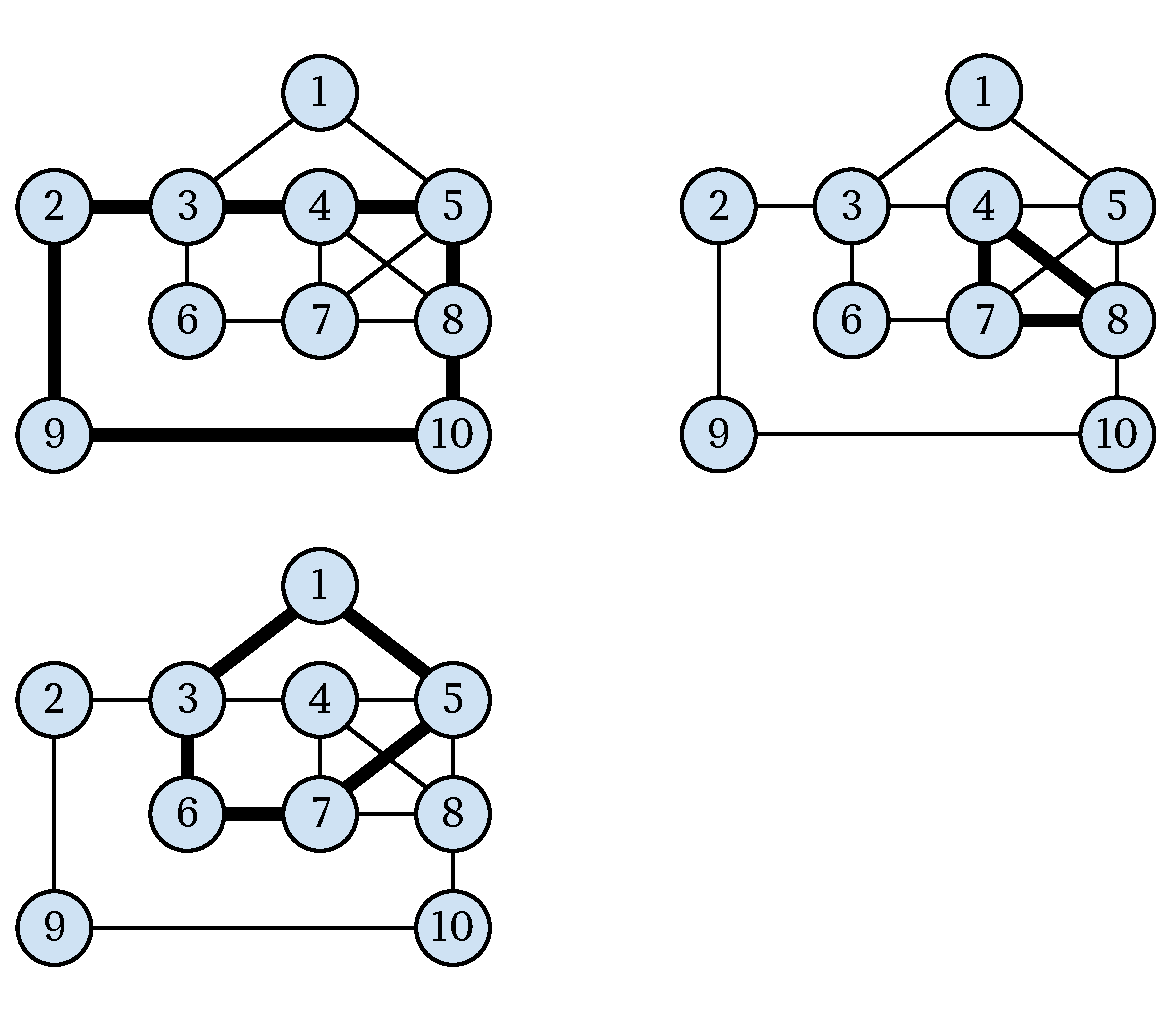
\includegraphics[width=7cm]{senior-example}

        Pane tähele, et on mitu võimalikku lahendust, nende hulgas ka
        selliseid, kus postiringe on ainult kaks.
    }

    \Scoring

    \begin{description}
        \item[Alamülesanne 1 (? punkti):] $3 \le N \le 2\,000$, $3 \le M \le 100\,000$.
        \item[Alamülesanne 2 (? punkti):] $3 \le N \le 100\,000$, $3 \le M \le 100\,000$.
        \item[Alamülesanne 3 (? punkti):] $3 \le N \le 500\,000$, $3 \le M \le 500\,000$.
    \end{description}

    \Constraints

    \begin{description}
        \item[Ajalimiit:] 0,5 s.
        \item[Mälulimiit:] 256 MB.
    \end{description}

\end{document}
